\section{$\lambdaLVar$: syntax and semantics}\label{s:lvars-lambdalvar}

The syntax of $\lambdaLVar$ appears in
Figure~\ref{f:lvars-lambdaLVar-syntax}, and
Figures~\ref{f:lvars-lambdaLVar-reduction-semantics}
and~\ref{f:lvars-lambdaLVar-context-semantics} together give the
operational semantics.  Both the syntax and semantics are
parameterized by the lattice $(D, \userleq, \bot, \top)$.

A \emph{configuration} $\config{S}{e}$ comprises a store and an
expression.  The \emph{error configuration}, written $\error$, is a
unique element added to the set of configurations, but
$\config{\topS}{e}$ is equal to $\error$ for all expressions $e$.  The
metavariable $\conf$ ranges over configurations.

Stores are as described in Section~\ref{subsection:lvars-stores}, and
expressions may be variables, values, function applications, @get@
expressions, @put@ expressions, or @new@.  The value forms include the
unit value $\unit$, elements $d$ of the specified lattice, store
locations $l$, threshold sets $T$, or $\lambda$-expressions
$\lam{x}{e}$.  A threshold set is a set $\setof{d_1, d_2, \dots}$ of
one or more elements of the specified lattice.

\FigLambdaLVarGrammar

\FigLambdaLVarReductionSemantics

\FigLambdaLVarContextSemantics

The operational semantics is split into two parts: a \emph{reduction
  semantics}, shown in
Figure~\ref{f:lvars-lambdaLVar-reduction-semantics}, and a
\emph{context semantics}, shown in
Figure~\ref{f:lvars-lambdaLVar-context-semantics}.

The reduction relation $\parstepsto$ is defined on
configurations. There are five rules in the reduction semantics: the
{\sc E-Beta} rule is standard $\beta$-reduction, and the rules {\sc
  E-New}, {\sc E-Put}/{\sc E-Put-Err}, and {\sc E-Get} respectively
express the semantics of the @new@, @put@, and @get@ operations
described in Section~\ref{subsection:lvars-communication-primitives}.
The {\sc E-New} rule creates a new binding in the store and returns a
pointer to it; the side condition $l \notin \dom{S}$ ensures that $l$
is a fresh location.  The {\sc E-Put} rule updates the store and
returns $\unit$, the unit value.  The {\sc E-Put-Err} rule applies
when a @put@ to a location would take its state to $\top$; in that
case, the semantics steps to $\error$.  The incompatibility of the
threshold set argument to @get@ is enforced in the {\sc E-Get} rule by
the $\incomp{T}$ premise, which requires that the lub of any two
distinct elements in $T$ must be $\top$.\footnote{Although
  $\incomp{T}$ is given as a premise of the {\sc E-Get} reduction rule
  (suggesting that it is checked at runtime), as \either{I}{we} noted earlier in
  Section~\ref{subsection:lvars-the-model-versus-reality}, in a real
  implementation of LVars threshold sets need not have any runtime
  representation, nor do they need to be written explicitly in the
  code.  Rather, it is the data structure author's responsibility to
  ensure that any operations provided for reading from LVars have
  threshold semantics.}

The context relation $\ctxstepsto$ is also defined on configurations.
It has only one rule, {\sc E-Eval-Ctxt}, which is a standard context
rule, allowing reductions to apply within a context.  The choice of
context determines where evaluation can occur; in $\lambdaLVar$, the
order of evaluation is nondeterministic (that is, a given expression
can generally reduce in more than one way), and so it is generally
\emph{not} the case that an expression has a unique decomposition into
redex and context.\footnote{In fact, \either{my}{our} motivation for splitting the
  operational semantics into a reduction semantics and a context
  semantics is to isolate the nondeterminism of the context semantics,
  which simplifies the determinism proof of
  Section~\ref{s:lvars-proof}.}  For example, in an application
$\app{e_1}{e_2}$, either $e_1$ or $e_2$ might reduce first.  The
nondeterminism in choice of evaluation context reflects the
nondeterminism of scheduling between concurrent threads, and in
$\lambdaLVar$, the arguments to @get@, @put@, and application
expressions are \emph{implicitly} evaluated concurrently.

\subsection{Fork-join parallelism}\label{subsection:fork-join}

$\lambdaLVar$ has a call-by-value semantics: arguments must be fully
evaluated before function application ($\beta$-reduction, via the {\sc
  E-Beta} rule) can occur.  We can exploit this property to define the
syntactic sugar @let par@ for \emph{parallel composition} that we first saw earlier in \eref{e:lvar-example-1}.  With @let par@, we can evaluate two subexpressions $e_1$ and $e_2$ in parallel before evaluating a third subexpression $e_3$:

\vspace{-8mm}
\singlespacing
\begin{displaymath}
\letparexp{x_1}{e_1}{x_2}{e_2}{e_3} \quad\defeq\quad \app{(\app{(\lam{x_1}{(\lam{x_2}{e_3})})}{e_1})}{e_2}
\end{displaymath}
\doublespacing

Although $e_1$ and $e_2$ can be evaluated in parallel, $e_3$ cannot be
evaluated until both $e_1$ and $e_2$ are values, because the
call-by-value semantics does not allow $\beta$-reduction until the
operand is fully evaluated, and because it further disallows reduction
under $\lambda$-terms (sometimes called ``full $\beta$-reduction'').
In the terminology of parallel programming, a @let par@ expression
executes both a \emph{fork} and a \emph{join}.  Indeed, it is common
for fork and join to be combined in a single language construct, for
example, in languages with parallel tuple expressions such as
Manticore~\cite{manticore_parallel_tuples}.

\begin{figure}[tb]
  \centering 
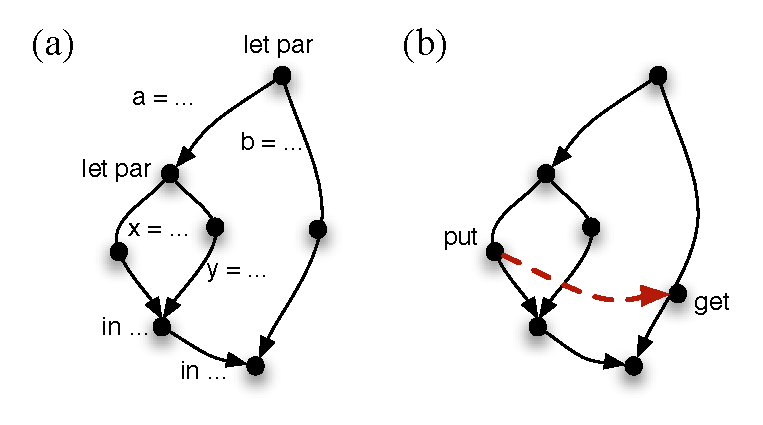
\includegraphics[width=4in]{chapter2/figures/lvars-series-parallel.pdf} 
\caption{A series-parallel graph induced by parallel
  $\lambda$-calculus evaluation (a); a non-series-parallel graph
  induced by \lstinline|put|/\lstinline|get| operations (b).}
  \label{f:lvars-series-parallel}
\end{figure}

Since @let par@ expresses \emph{fork-join} parallelism, the evaluation
of a program comprising nested @let par@ expressions would induce a
runtime dependence graph like that pictured in
Figure~\ref{f:lvars-series-parallel}(a).  The $\lambdaLVar$ language
(minus @put@ and @get@) can support any \emph{series-parallel}
dependence graph.  Adding communication through @put@ and @get@
introduces ``lateral'' edges between branches of a parallel
computation, as in Figure~\ref{f:lvars-series-parallel}(b).  This adds
the ability to construct arbitrary non-series-parallel dependency
graphs, just as with \emph{first-class
  futures}~\cite{beyond-nested-workstealing}.

Because we do not reduce under $\lambda$-terms, we can sequentially
compose $e_1$ before $e_2$ by writing $\letexp{\_}{e_1}{e_2}$, which
desugars to $\app{(\lam{\_}{e_2})}{e_1}$.  Sequential composition is
useful for situations in which expressions must run in a particular order,
\eg, if we want to first allocate a new LVar with @new@ and then write to it
using @put@.

\subsection{Errors and observable determinism}\label{subsection:lvars-errors-and-observable-determinism}

Is the @get@ operation deterministic?  Consider two lattice elements
$d_1$ and $d_2$ that have no ordering and have $\top$ as their lub,
and suppose that @put@s of $d_1$ and $d_2$ and a @get@ with
$\setof{d_1, d_2}$ as its threshold set all race for access to an LVar
$lv$:

\vspace{-8mm}
\singlespacing
\begin{equation}
\begin{split}
& \LETPAR ~\_ = \putexp{\mathit{lv}}{d_1} \\
&  \letparspace ~\_ = \putexp{\mathit{lv}}{d_2} \\
&  \letparspace ~x = \getexp{\mathit{lv}}{\setof{d_1, d_2}} \\
&  \letspace \IN~x
\end{split}
\label{e:lvar-example-5}
\end{equation}
\doublespacing

Eventually, \eref{e:lvar-example-5} is guaranteed to raise $\error$ by way of the
{\sc E-Put-Err} rule, because $\userlub{d_1}{d_2} = \top$.  Before
that happens, though, $\getexp{lv}{\setof{d_1, d_2}}$ could return
either $d_1$ or $d_2$.  Therefore, @get@ \emph{can} behave
nondeterministically---but this behavior is not observable in the
final outcome of the program, since one of the two @put@s will raise
$\error$ before the $x$ in the body of the @let par@ can be evaluated, and under
our definition of observable determinism, only the final outcome of a
program counts.

